\documentclass{VUMIFPSkursinis}
\usepackage{algorithmicx}
\usepackage{algorithm}
\usepackage{algpseudocode}
\usepackage{amsfonts}
\usepackage{amsmath}
\usepackage{bm}
\usepackage{caption}
\usepackage{color}
\usepackage{float}
\usepackage{graphicx}
\usepackage{listings}
\usepackage{float}
\usepackage{subfig}
\usepackage{wrapfig}
\usepackage[hidelinks]{hyperref}
\usepackage{todonotes}

% Titulinio aprašas
\university{Vilniaus universitetas}
\faculty{Matematikos ir informatikos fakultetas}
\department{Programų sistemų katedra}
\papertype{Programų kūrimo proceso laboratorinis darbas}
\title{Įmonės ,,Mėnuliukų technologijos" programų kūrimo proceso aprašas (Pirmas laboratorinis darbas)}
\titleineng{Description of the development process of the ,,Moon technologies" company (First laboratory work)}
\status{4 kurso 3 grupės studentai}
\author{Matas Savickis, Justas Tvarijonas, Džiugas Mažulis}
\secondauthor{Greta Pyrantaitė, Andrius Bentkus}


\supervisor{Saulius Ragaišis, Doc., Dr.}
\date{Vilnius – \the\year}

% Nustatymai
% \setmainfont{Palemonas}   % Pakeisti teksto šriftą į Palemonas (turi būti įdiegtas sistemoje)
\bibliography{bibliografija}

\begin{document}
\maketitle

\tableofcontents

\sectionnonum{Įvadas}
	Šiame darbe bus pristatytas ,,Mėnuliukų technologijų" programų kūrimo procesas.
	Pats procesas yra paremtas Agile metodologija su minimaliais pakeitimais reikalavimų rinkime.
	Proceso pradžioje stengiamės su užsakovu išsiaiškinti norimus įgyvendinti funkcionalumus ir bendraujant kartu su užsakovu sudaryti reikalavimus. 
	Sudarant reikalavimus yra diskutuojama ir sistemos ateities vizija siekiant susidaryti geresnę perspektyvą sistemos ateičiai ir darbartiniams reikalavimams.
	Įmonė įvertina kiek valandų užtruks kiekvieno funkcionalumo sukūrimas ir mokestis yra imamas už pradirbtas valandas.
	Klientui nesutikus su pateiktomis kainomis yra daromi susitikimai siekiant paaiškinti valandų vertinimą. Po susitikimų funkcionalumo įgyvendinimo valandos gali keistis, arba funkcionalumas bus atsisakytas.

\section{Kūrimo procesas}
\todo[inline]{Pridėti acceptance testing cikle su programavimu. Iš kokybės užtikrino proceso gali atsirasti naujas defektas.}
	\begin{figure}[htbp]
	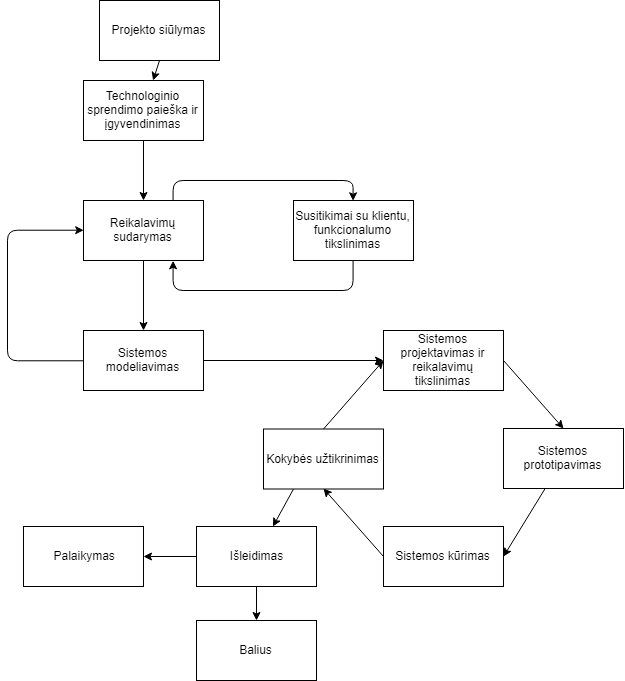
\includegraphics[scale=0.6]{img/SoftwareProcessMoonTechnologies}
	\caption{Sistemos kūrimo procesas} % Antraštė įterpiama po paveikslėlio
	\label{img:kurimoProcesas}
	\end{figure}
	\subsection{Projekto siūlymas}

	\begin{center}
		\begin{table}[ht]
			\caption{Projekto siūlymo procesas}
		\begin{tabular}{ | l | l | } 
		\hline
	Pavadinimas:         & Projekto siūlymas.                                      \\ \hline
	Tikslas: 	           & Aptarti galimą projektą su galimu klientu. 							\\ \hline
	Vykdytojai:          & Projekto vadovas ir klientas.                             \\ \hline
	Veiklos:             & V1 - Aptariama sistemos aprėptis. 													\\
											 & V2 - Nustatomos kainos ribos iki pirmo sistemos išleidimo.  \\
											 & V3 - Pirminės sutarties pasirašymas 													\\ \hline
	Naudojami produktai: & NP1 - Buvusių projektų dokumentai. 													 \\ \hline
	Sukuriami produktai: & SP1 - Pirminė sutartis sistemos projektavimui. 								\\ \hline
\end{tabular}
\end{table}
\end{center}
\begin{enumerate}
	\item Pirmas susitikimas, kuriame aptariamas galimas projektas, kiekviena pusė išsako savo lūkesčius, pasidalinama įdėjomis.
	\item Po susitikimo įmonė paruošia pradininį pasiūlymą, į kurį įeina orientacinės finansų ribos, žmonių ištekliai, kurie galėtų būtų skiriami šiam projektui. Šis pasiūlymas aptariamas su klientu, kartu su juo dokumentuojami funkcionalumai, kurių klientas nori pirmame sistemos išleidime. Sėkmingai tesiantis tolesnėms deryboms nutariama dėl pradinio technologinio sprendimo pasiūlymo datos, bei finansavimo jam.
	\item Pasirašoma pradinė sutartis, kurioje dokumentuojama prieš tai aptarta informacija. Ši sutartis galioja iki pirmojo prototipo pasiūlymo, po kurio atnaujinamos derybės dėl tolesnio projekto vystymo.
\end{enumerate}

	\subsection{Technologinio sprendimo paieška ir įgyvendinimas}
	\todo[inline]{update}
		Pasirašius sutartį su klientu pradedama ieškoti konkretaus technologinio sprendimo tinkamo projekto vystimui. Sutatomos konrečios karkasų, duomenų bazių arba betkokios kitos technologijos versijos kurios bus naudojamos. Jeigu projektas yra jau egzistuojantis ir klientas perka tolimesnį projekto vystimą yra išsiaiškinama ar nereikės pakelti projekte naudojamų technologijų versijos.
		Projektuojant sistema siekiama patenkinti arba siekti išvardintas charakteristikas:
	\begin{itemize}
		\item{
			Intersuotų asmenų įvairovė - sistema turis patenkinti įvairių interesuotų asmenų norus ir poreikius, pavyzdžiui vadovai, savininkai, vartotojai ir valdytojai.
			%Kiekvienas interesuotas asmuo turi savo asmeninius interesuosus, kuriuos nori įvykdyti naudodamasis asmeninius interesuosus, kuriuos nori įvykdyti naudodamasis sistemą.
			%"Mėnuliukų technologijos" kompanijoje atidžiai ir glaustai bendraujama su interesuotais asmenimis tam kad tiksliai ir akivaizdžiai išsaiškinti interesuotais.
		}
		\item{Interesų atskyrimas - bandoma atskirti interesai taip, kad lengviau būtų realizuoti galutinėje sistemoje.  }
		\item{Remiamasi kokybės užtikrinimu - Bandoma taip pat siekti nefunkcinių reikalavimų užtikrinimu pavyzdžiui užtikrinti greitaveiką.}
	\end{itemize}
	
	\subsection{Reikalavimų ciklas}
	\todo[inline]{update}
		Nutarus dėl konkrečių technologijų, kurios bus naudojamos pradedame funkcinių ir nefunkcinių reikalavimų sudarymas. Jų sudarymas vyksta cikliškai, pirma mūsų įmonės verslo analitikas išanalizuoja verslo poreikius ir kartu su architektu sudaro pirminius reikalavimus, jie yra pristatomi klientui kartu su klausimais, įvyksta suformuotų reikalavimų aptarimas. Aptarime dalyvauja architektas, verslo analistas ir verslo žmogus. Jeigu klientas sutinka su sudarytais reikalavimais pradedamas sistemos modeliavimas, jeigu kyla neaiškumų dėl reikalavimų tarp kliento ir mūsų įmonės grįžtama prie poreikių sudarimo įmonės viduje. Ciklas vyksta iki tol kol pasiekiamas sutarimas tarp mūsų įmonės ir kliento.
	\subsection{Sistemos modeliavimas}
	\begin{figure}[H]
	\centering
	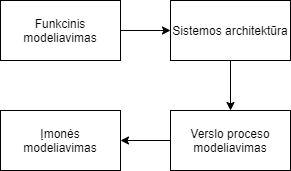
\includegraphics[scale=0.7]{img/SistemosModeliavimas}
	\caption{Sistemos modeliavimas} % Antraštė įterpiama po paveikslėlio
	\label{img:mlp}
	\end{figure}
		Modeliavimas vykdomas Ad-hock principu, pasitelkiant praeities žinias arba tiesiog susėdus ekspertams ir bandant išsiaiškinti sprendimą.
		Programų kūrimo proceso modeliavimą sudaro keturios dalys:
		\begin{enumerate}
		\item Sistemos architektūra - šiame žingsnyje apibrėžiama sąveiką tarp skirtingų sistemos komponentų(duomenų bazių, servisų ir kitą) bei išorinių sistemų. Šiam modeliavimui pasitelkta UML komponentų diagramos. Sistema yra išskaidoma į skirtingus \hyperref[mikro]{mikroservizus}
		\item Verslo proceso modeliavimas - šiam modeliavimui naudojami BPMN grafifai apibrėžentys verslo procesus. Sukurti procesai analizuojami, tobulinami. Taip pat išskiriamos verslo proceso dalys kurias galima automatizuoti.
		\item Įmonės modeliavimas - abstrakčiai sumodeliuojama kaip įmonės procesai įtakos tolimesnį programos vystymą. 
			Kokie procesų modeliai reikalingi sukurti pseudo kodui. Iš procesų modelių ir duomenų modelių kyla reikalavimai.
		\end{enumerate}
		\subsubsection{Mikroservisai}
		\todo[inline]{Šitą matyt šalinam?}
		\label{mikro} 
		"Mėnuliukų technologijos" bando atskirti bendrą sistemą į daug mažesnių sistemų remdamasi dabartine populiaria mikroservisu architektūra.
		Kiekviena atskirta sistema turi būti kuo savarankiškesnė ir atlikti būtent vieną funkcionalumą, tačiau jį turės atlikti kuo efektyviau.
		Mikroservisai turi itin aiškiai apibrėžtas programų sąsajas bei dokumentaciją, kuri akivaizdžiai apibrėžia funkcionalumą.
		Taip užtikrinama, jog programų sistemos tikslingai atlieka reikalaujamus verslo siekius.

		\begin{figure}[H]
		\centering
		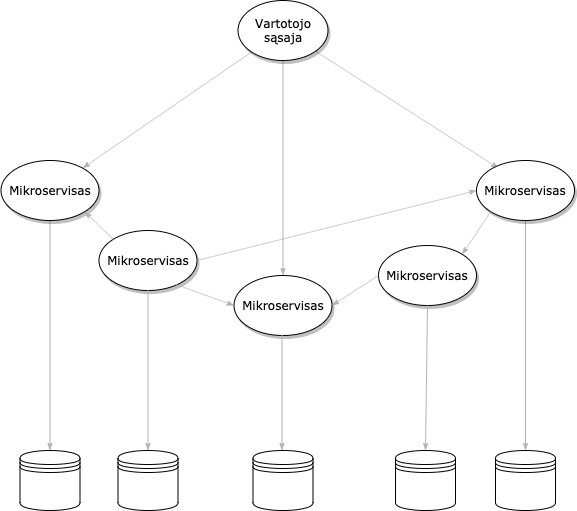
\includegraphics[scale=0.6]{img/micro.png}
		\caption{Mikroservisų architektūra}
		\label{img:mikroservizai}
		\end{figure}
		Mikroservisų architektūros teikiami privalumai:
		\begin{itemize}
			\item{atskiros sistemos dalys yra lengviau prižiūrimos ir lengviau testuojamos}
			\item{silpna sistemos sąsajo - neglaudus sąryšis tarp komponentų bei programų leidžia daryti pakeitimus, kurie nepropaguoja per visą sistemą}
			\item{nepriklausomas servisų dalis galima atskirai diegti bei atlikti atnaujinimus nediegiant visos sistemos iš naujo}
			\item{Mažos komandos efektyviau prižiūri sistemą, reikia mažiau komunikacijos}
			\item{Servisai kuriami pagal įmonės gebėjimus}
		\end{itemize}
		
	\subsection{Sprintas}
	Sprintu skaitome dvi savaites, kurių pabaigoje yra įvykdytas verslo analitiko ar komandos parinktas užduočių skaičius ir matomas apčiuopiamas rezultatas - veikiantis funkcionalumas. Sprinto ilgis - 2 savaitės - pasirinktas taip, kad nebūtų sunku numatyti ir suplanuoti užduočių tam laiko tarpui ir taip, kad būtų pakankamai laiko jas įvykdyti iki galo. Sprintas turi kelias veiklas, kurios skirtos palaikyti efektyvią programos kūrimo eigą ir užtikrinti, kad rezultatas būtų pasiektas laiku.
	\subsubsection{Sprinto užduočių tikslinimas ir vertinimas}
	\begin{center}
		\begin{table}[ht]
			\caption{Sprinto užduočių tikslinimo ir vertinimo procesas}
		\begin{tabular}{ | l | l | } 
		\hline
	Pavadinimas:         & Sprinto užduočių tikslinimas ir vertinimas.          		 					 \\ \hline
	Tikslas: 	           & Įvertinti ir paanalizuoti užduotis. 																	\\ \hline
	Vykdytojai:          & Programuotojas bei Įmonės analistas arba užsakovo atstovas, klientas  \\ \hline
	Veiklos:             & V1 - Analistas paaiškina užduotis iš verslo perspektyvos. 		          \\
											 & V2 - Užduočių vertinimo sesija tarp programuotojų.					             \\
											 & V3 - Įvertintų užduočių aptarimas su analistu 									          \\ \hline
	Naudojami produktai: & NP1 - Užduočių sąrašas. 													 							           \\ \hline
	Sukuriami produktai: & SP1 - Sprinto užduočių sąrašas. 																	          \\ 
											 & SP2 - Įvertintos užduotys backloge(vertimas?) 										           \\ \hline
\end{tabular}
\end{table}
\end{center}
\begin{enumerate}
	\item Pradinis užduočių aptarimas su analistu arba užsakovo atstovu, šiame aptarime paaiškinami kiekvienos užduoties scenarijai iš dalykinės srities pusės, paaiškinami reikalavimai, kurie turi būti įgyvendinami prieš pabaigiant užduotį. Diskusijos su programuotojais metu galimi užduočių ar jų priėmimo kriterijų pakeitimai arba, jeigu jų negalima atlikti nepasitarus su klientu, užduotis yra atnaujinama vėliau, pasitarus su klientu.
	\item Atlikus pradinį aptarimą kartu su analistu arba verslo atstovu rengiama diskusija tarp programuotojų, kuriame kiekviena užduotis yra įvertinama taškais, vertinama fibonačio sekos skaičiais, o skaičiaus reikšmė yra viena programuotojo darbo diena. Šioje diskusijoje programuotojai diskutuoja apie galimą kiekvienos užduoties implementaciją, bei jos sudėtingumą, tada balsuojama dėl šiai užduočiai skiriamo balų skaičiaus. Taip aptariamos visos dar neįvertintos užduodys, tuo atvėju, jeigu gilinantis į implementaciją atsiranda neaiškumų dėl dalykinės srities, užduotis yra blokuojama paliekant komentarą, kad jį radęs analistas galėtų patikslinti užduotį.
	\item Atlikus užduočių vertinimą analistas arba verslo atstovas sudeda sekančio sprinto struktūra pagal galimą talpą (talpa lygi programuotojų skaičiui padauginta iš 8). 
\end{enumerate}
\todo[inline]{Ką darom su šitu tekstu? Tekstas gražus, bet nežinau kaip įkomponuot.}
	Tai viena svarbiausių fazių, kadangi jos kokybiškas įvykdymas padeda pagrindą visam spintui -  jei reikalavimai netikslūs ar užduotys prastai aprašytos ir jų sudėtingumas atmestinai įvertintas - sprintas pasmerktas nesusipratimams ir laiko gaišimui aiškinantis, koks sprinto tikslas ir koks jo sėkmingo baigimo vertinimas. Sprinto reikalavimų tikslinime ir vertinime dalyvauja komanda ir verslo analitikas. Verslo analitikas pateikia reikalavimus ir išskirtas užduotis, kartu su komanda tikslina priėmimo kriterijus tol, kol susidaro pilnos užduotys su tiksliais užduoties sėkmingo įvykdymo reikalavimais ir klausimais klientui jei iškyla neaiškumų. Komanda taip pat įvertina aptariamų užduočių sudėtingumą ir kartu su verslo analitiku nusprendžia, kokias ir kiek užduočių įdėti į sekantį sprintą.
	\subsubsection{Užduočių analizė}
	\todo[inline]{Update}
	Turint pilnai aprašytas užduotis vyksta užduočių analizė, jei yra tam poreikis. Jei kyla daugiau neiškumų dėl projekto vykdymo ateities planų gali būti sukuriamos atskiros užduoties tam tikros srities išsiaiškinimui tam, kad geriau išsiaiškinti galimas implementacijos alternatyvas. Tokios analizės rezultatas - dokumentas, pateikiantis klausimus ir atsakymus, implementacijos alternatyvas ir kilusius kitus pastebėjimus. Po analizės turi būti aišku, kaip ir su kokiomis technologijomis užduotis bus įvykdoma ir, jei reikalinga, tikslinamos užduotys. 
	\par Jei analizė reikalinga mažesniu mastu, bet dar negalima iškart imti ir programuoti - asmeniškai, jau pasiėmus užduotį, aiškinamasi, kokių žinių trūksta ir kas jas galėtų suteikti. Tai gali būt pasikalbėjimas su kolegomis ar panašių užduočių implementacijos pavyzdžių ieškojimas. Šios veiklos pabaigoje jau galima pradėti progamuoti.
	\subsubsection{Programavimas}
	\todo[inline]{Update}
	Šis žingsnis glaudžiai susijęs su prieš jį einančiomis fazėmis, jame vykdomas suprojektuotos sistemos dalies įgyvendinimas, kuris apima kodo rašymą, automatizuotų testų kūrimą, konfigūracijos pakeitimus ir duombazės kūrimą. Ši fazė įgyvendinama tik gerai išsiaiškinus ir susidokumentavus reikalavimus ir jau turint prototipą, kad kuriama programa atitiktų kliento lūkesčius ir reikalingų pakeitimų būtų mažiau.
	\subsubsection{Kokybės užtikrinimas}
	\todo[inline]{Papildyt aprašymą po lentele, pridėt automated testing.}
	\begin{center}
		\begin{table}[ht]
		\caption{Kokybės užtikrinimo procesas}
		\begin{tabular}{ | l | l | } 
		\hline
		Pavadinimas:         & Kokybės užtikrinimas.                                       \\ \hline
		Tikslas: 	           & Patikrinti sistema su atnaujinta kodo baze veikia teisingai. \\ \hline
		Vykdytojai:          & Testuotojai ir programuotojai.                                \\ \hline
		Veiklos:             & V1 - Leidžiami integraciniai testai. 													\\
						             & V2 - Testų klaidų analizė ir defektų sūkurimas. 								 \\
					 	             & V3 - Testų rezultatų apibendrinimas. 														\\ 
						    				 & V4 - Performance testavimas. 																		 \\ \hline
		Naudojami produktai: & NP1 - Integraciniai testai. 																				\\
												 & NP2 - ?																													 \\ \hline
		Sukuriami produktai: & SP1 - Nauji defektai. 																								\\
												 & SP2 - Testų rezultatų dokumentas 																	 \\
												 & SP3 - Performance analizės dokumentas. 															\\ \hline
		\end{tabular}
	\end{table}
		\end{center}
	Kokybės užtikrinimas skirtingas kiekvienam projektui. Tuose projektuose, kuriuose kuriamoje sistemoje egzistuoja vartotojo sąsaja, atliekamas rankinis testavimas kartu su automatizuotu regresiniu testavimu. Į kokybės užtikrinimą yra įtraukiami ir programuotojai, kurie yra atsakingi už automatizuotų testų teisingumą. Testuotojai atsakingi už rankinį testavimą bei regresinių testų rezultatų apibendrinimą. Jeigu projektas yra iteracinis ir jau išleistas plačiam naudojimui, po sėkmingo testavimo kodas yra sudedamas į aukštesnę aplinką, kurioje yra papildomai pravaliduojamas prieš jį išleidžiant į produkciją.
	\subsubsection{Konfigūracijos valdymas}
	\todo[inline]{Update. Nutart, kas pas mus yra konfigūracijos valdymas.}
	Užtikrinant didesnį sistemos patikimumą reikalingos skirtingos aplinkos skirtos testuoti sistemą, šioms aplinkoms palaikyti atliekamas konfigūracijos valdymas - kiekvieno sprinto metu konfigūracijoje ar duomenų bazėje atliktus pakeitimus programuotojas pažymi tam skirtoje vietoje, pagal kurią po sprinto devOps specialistai atlieka konfigūracinius pakeitimus aplinkose, kuriose šie pakeitimai reikalingi. Taip pat po sprinto kodas yra sudedamas į aukštenę aplinką tolimesniam testavimui.
	\subsubsection{Sprinto aptarimas}
	\todo[inline]{Update. Kas dalyvauja?}
	Komandos efektyvumui labai svarbu aptarti praėjusį sprintą: kas trukdė efektyviam darbui, kas gerai sekės, kokias programavimo veiklas tęsti, kokias nutraukti, kokios komandos nuotaikos ir to priežastys. Šios veiklos rezultatas - pagal išreikštus pastebėjimus išskirti tobulėjimo punktai, kurių laikomasi būsimame sprinte siekiant geresnės ir greitesnės projekto implementacijos. Tai gali būti aktyvus kažkokių procesų vykdymo trukdžių sprendimas, komunikacija su kitomis komandomis ar klientu dėl iškilusių problemų.
	\subsubsection{Defekto analizė}
	\todo[inline]{Update}
	Defekto analizės procesas pradedamas problemos identifikavimu. Vartotojo arba testuotojo aptikas defektas yra užregistruojamas aprašant sąlygas, reikalingas atkurti defektą, bei priskiriamas atitinkamai defektų klasei. Programuotojas išanalizuoja defektą, suranda defekto priežastį bei apibrėžia ir įgyvendina priežasčiai išspręsti reikalingą veiksmų seką. Įgyvendinus šiuos žingsnius belieka įsitikinti, kad procesas atnešė pageidaujamą rezultatą - defektas nurodytomis sąlygomis neegzistuoja.

	\subsection{Išleidimas}
	\todo[inline]{Update}
	Išleidimo stadiją galima skaidyti į 2 skirtingus tipus - galimas naujas projekto išleidimas, kurio metu vartotojui pateikiama nauja sistema, kuri buvo tam tikrą laiką kuriama. Taip pat egzistuoja kitas variantas, kai yra veikianti sistema, kuri yra atnaujinama kas tam tikrą laiką (tai priklauso nuo sprinto ilgi). Išleidimo metu įmonėje yra vykdomi darbuotojų budėjimai, kad sistemai veikiant ne tiksliai pagal planą, sistemos trikdžiai būtų kuo greičiau pašalinti.
	\subsection{Palaikymas}
	\todo[inline]{Update}
	Palaikymo procesui kuriamas palaikymo planas, susidedantis iš programos paruošimo, problemos identifikavimo bei produkto konfigūracijos valdymo. Problemos identifikavimas vykdomas tikrinant programos validumą, sukuriant problemos sprendinį bei išskiriant resursus modifikacijai įgyvendinti. Proceso patvirtinimas įgyvendinamas gavus patvirtinimą dėl kėtinamų įgyvendinti pakeitimų  iš užklausos autoriaus. Įmonė teikia dviejų tipų palaikymą: taisomąjį bei adaptacinį. Taisomasis palaikymas orientuotas į problemų, atrastų vartotojų arba vartotojų klaidų reportų analizės metu, taisymą. Adaptacinis palaikymas skirtas nūdienos standartų programose palaikymui. Įmonė laikosi „Boehm“ modelio, kuris pasižymi atitinkamai pakeitimų pasiūlymu, patvirtinimu bei įgyvendinimu.
	\label{img:boehmsModel} 

	\subsection{Balius/Post-mortem}
	Procesas užbaigiamas komandos bei prie projekto prisidėjusių žmonių švente, kurioje aptariamas bei įvertinamas proceso pasisekimas ir daromos išvados.

\sectionnonum{Rezultatai ir išvados}
\todo[inline]{Ar šito skyriaus čia iš vis reikia?}
\todo[inline]{Šarūnas minėjo, kad Ragaišis visai glossary nori.}



\end{document}
